\section{A general overview}
\subsection{Where does it come from?}

\begin{frame}
  \frametitle{The nature}
  \begin{block}{Natural Selection}
    \begin{itemize}
    \item Darwin\cite{darwin.1840.origin.of.species} introduces
      Natural selection.
    \item It implies several conditions:
      \begin{itemize}
      \item Reproduction of individuals in the population.
      \item Variation that affects the likelihood of survival of
        individuals.
      \item Heredity in reproduction.
      \end{itemize}
    \end{itemize}
  \end{block}

  \begin{block}{Sexual/Asexual?}
    \begin{itemize}
    \item Asexual reproduction is based on cloning, and
      eventually mutation.
    \item Sexual is based on crossover.
    \end{itemize}
  \end{block}
\end{frame}

\begin{frame}
  \frametitle{Link with Genetic Programming?}
  \begin{block}{On the idea}
    \begin{itemize}
    \item Make evolve a population to solve a problem.
    \item The population could be a lot of things(programs, parameters\dots).
    \end{itemize}
  \end{block}

  \begin{block}{On the way its done}
    \begin{itemize}
    \item Create the population,
    \item Choose the best,
    \item Keep only the best,
    \item Make them create a new generation,
    \item And so on until the population solves the problem.
    \end{itemize}
  \end{block}
\end{frame}


\begin{frame}
  \frametitle{A basis graphical overview}
  \begin{center}
    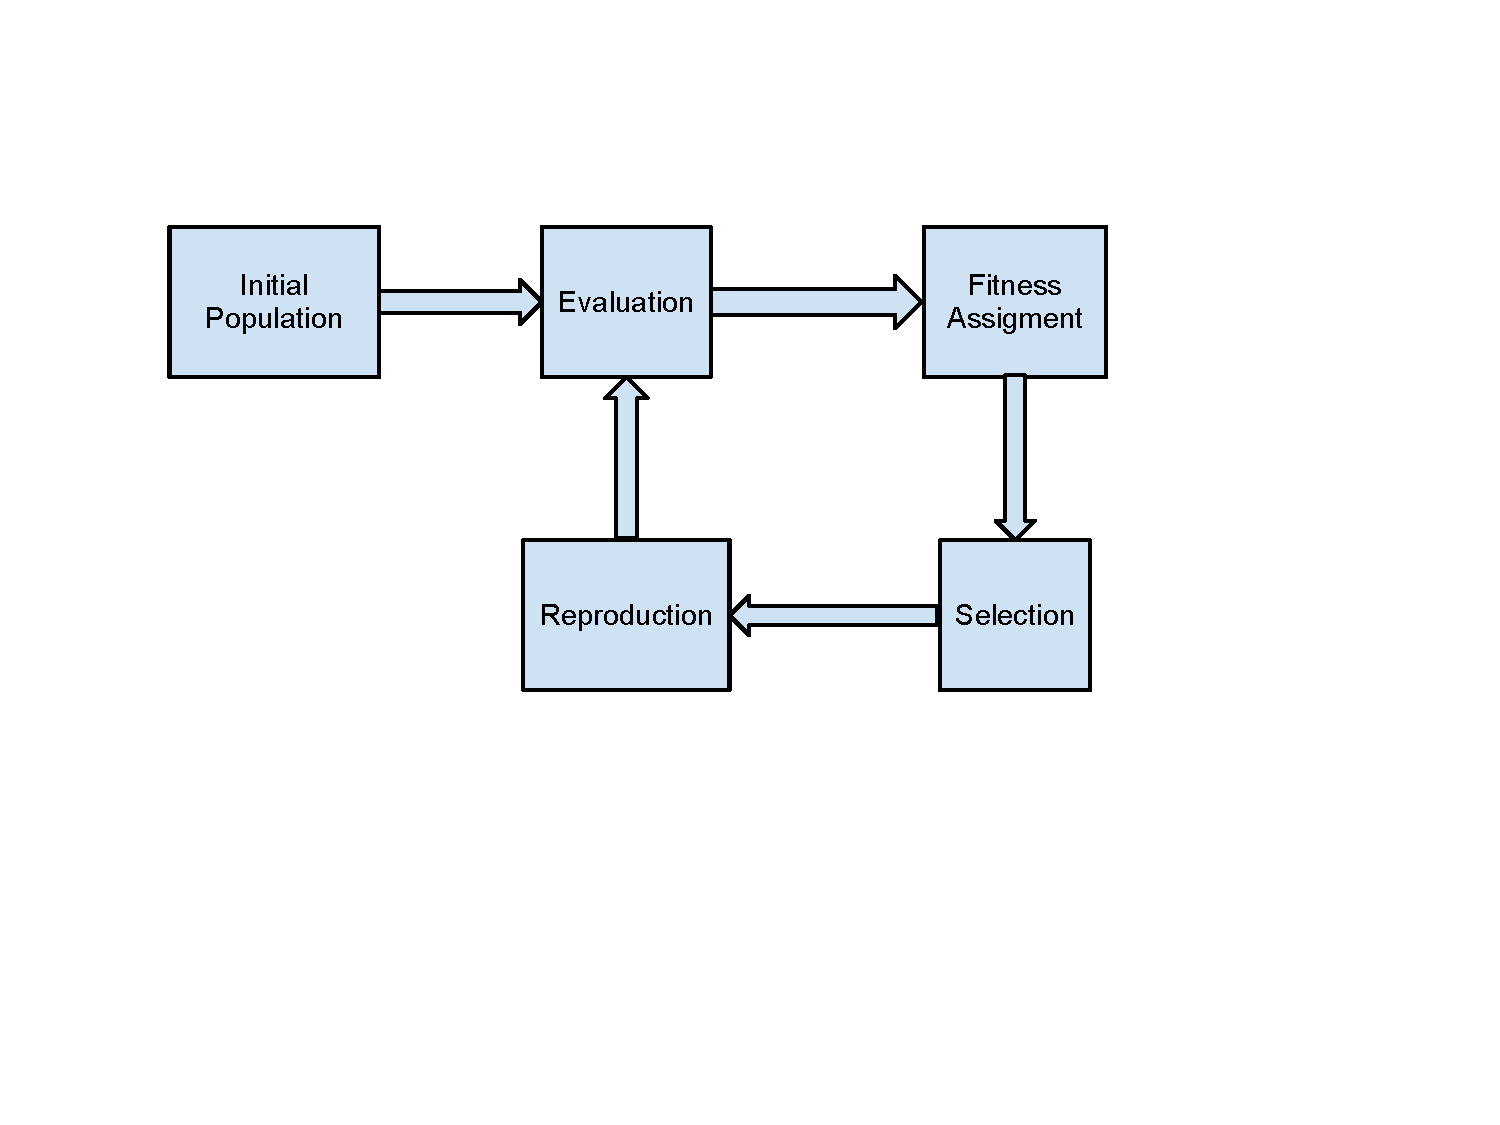
\includegraphics[scale=0.5]{img/cycle}
  \end{center}
\end{frame}

\subsection{Definitions}

\begin{frame}
  \frametitle{EA, GA, GP, ES... ???}
  \begin{block}{In the literature}
    \begin{itemize}
    \item When you are looking for genetic programming, you'll find a
      lot of different things.
    \item In this talk, we consider Evolutionary Algorithm as an
      umbrella term to represent techniques which use evolution.
    \end{itemize}
  \end{block}

  \begin{center}
    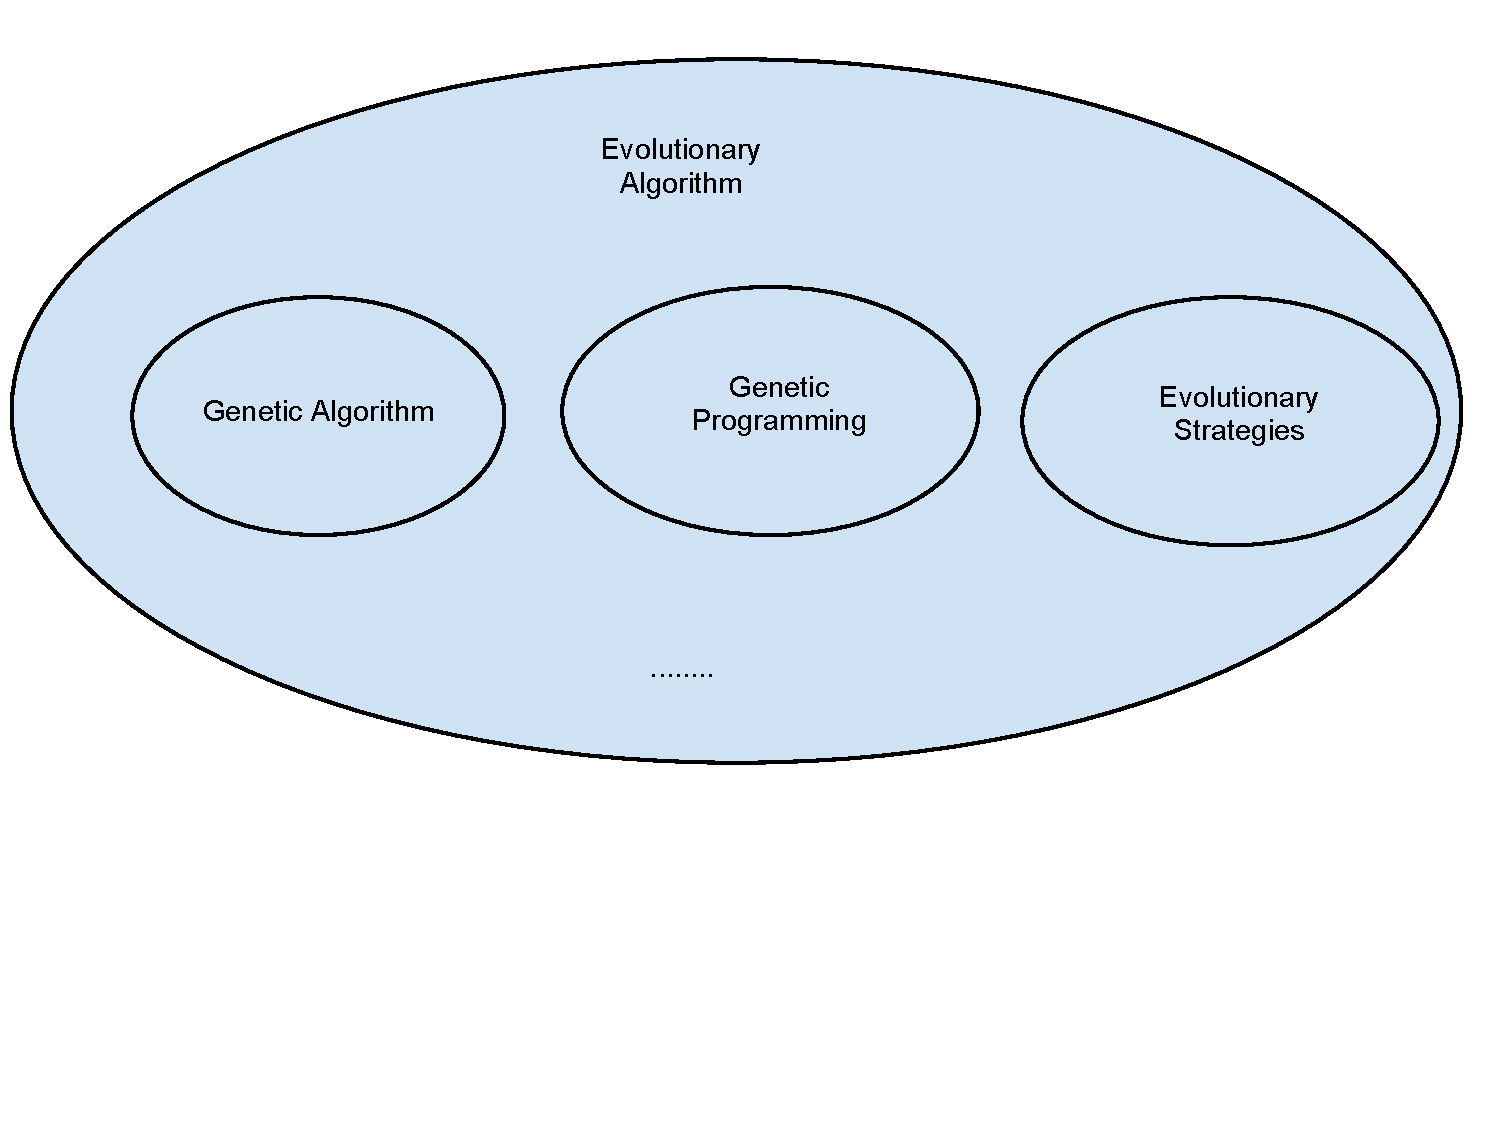
\includegraphics[scale=0.4]{img/ea}
  \end{center}
\end{frame}

\begin{frame}
  \frametitle{Genetic Algorithms}
  \begin{block}{History}
    \begin{itemize}
    \item Developed by Holland\cite{holland1992}.
    \item The original GA uses:
      \begin{itemize}
        \item fixed-length binary representation.
        \item Crossover a lot.
      \end{itemize}
    \item This model has been extended, now GA uses an alphabet (like DNA).
    \item We'll let the theoretical development for the second part.
      %% In this phrase, I mean Pierre, you have to explain the GA 1-point
      %% crossover (GP An introduction p96) and the schemata.
    \end{itemize}
  \end{block}
\end{frame}

\begin{frame}{Genetic Algorithms (cont.)}
  \begin{algorithm}[H]
    \caption{Genetic Algorithm}
    \begin{algorithmic}
      \State t := 0
      \State initPopulation P(t)
      \State evaluate P(t)
      \While {not done}
        \State ++t
        \State P' := selectParents P(t)
        \Comment{Crossover}
        \State recombine P'(t)
        \State mutate P'(t)
        \State evaluate P'(t)
        \State P := survive P', P(t)
      \EndWhile
    \end{algorithmic}
  \end{algorithm}
\end{frame}

\begin{frame}
  \frametitle{Evolutionary Strategies}
  \begin{block}{History}
    \begin{itemize}
    \item Idea started in 1960.
    \item Defined by Rechenberg\cite{Rechenberg.1975} and Schwefel\cite{Schwefel.1981}.
    \end{itemize}
  \end{block}

  \begin{block}{Characteristics}
    \begin{itemize}
    \item Only mutation.
    \item Coma-evolution: All parents died before selection.
    \item Plus-evolution: All are considered for selection.
    \item In the selection: each generation is more little than the
      precedent.
    \end{itemize}
  \end{block}
\end{frame}


\begin{frame}
  \frametitle{Evolutionary Programming}
  \begin{block}{History}
    \begin{itemize}
      \item Created in 1966, by Fogel, Owens, and Walsh\cite{fogel1966}.
    \end{itemize}
  \end{block}

  \begin{block}{Characteristics}
    \begin{itemize}
    \item Works on Finite-State Machine.
    \item Can modify: initial state, number of states, transition\dots
    \item Mutation decreases as the optimal fitness approaches.
    \end{itemize}
  \end{block}
\end{frame}


\begin{frame}
  \frametitle{Genetic Programming}
  \begin{block}{History}
    \begin{itemize}
    \item Works on program instead of parameters.
    \item Introduced by Koza\cite{Koza92}.
    \item Works on parse-tree.
    \end{itemize}
  \end{block}

  \begin{block}{Characteristics}
    \begin{itemize}
    \item Many people uses LISP.
    \item We can found assembly language too.
    \item Example: can find the function $x^2/2$.
    \end{itemize}
  \end{block}
\end{frame}


%%% Local Variables:
%%% mode: latex
%%% mode: flyspell
%%% TeX-master: "../genetic"
%%% ispell-dictionary: "en"
%%% compile-command: "cd .. && make"
%%% End:
